\documentclass{standalone}
\usepackage{tikz}
\usetikzlibrary{patterns, positioning}


\begin{document}
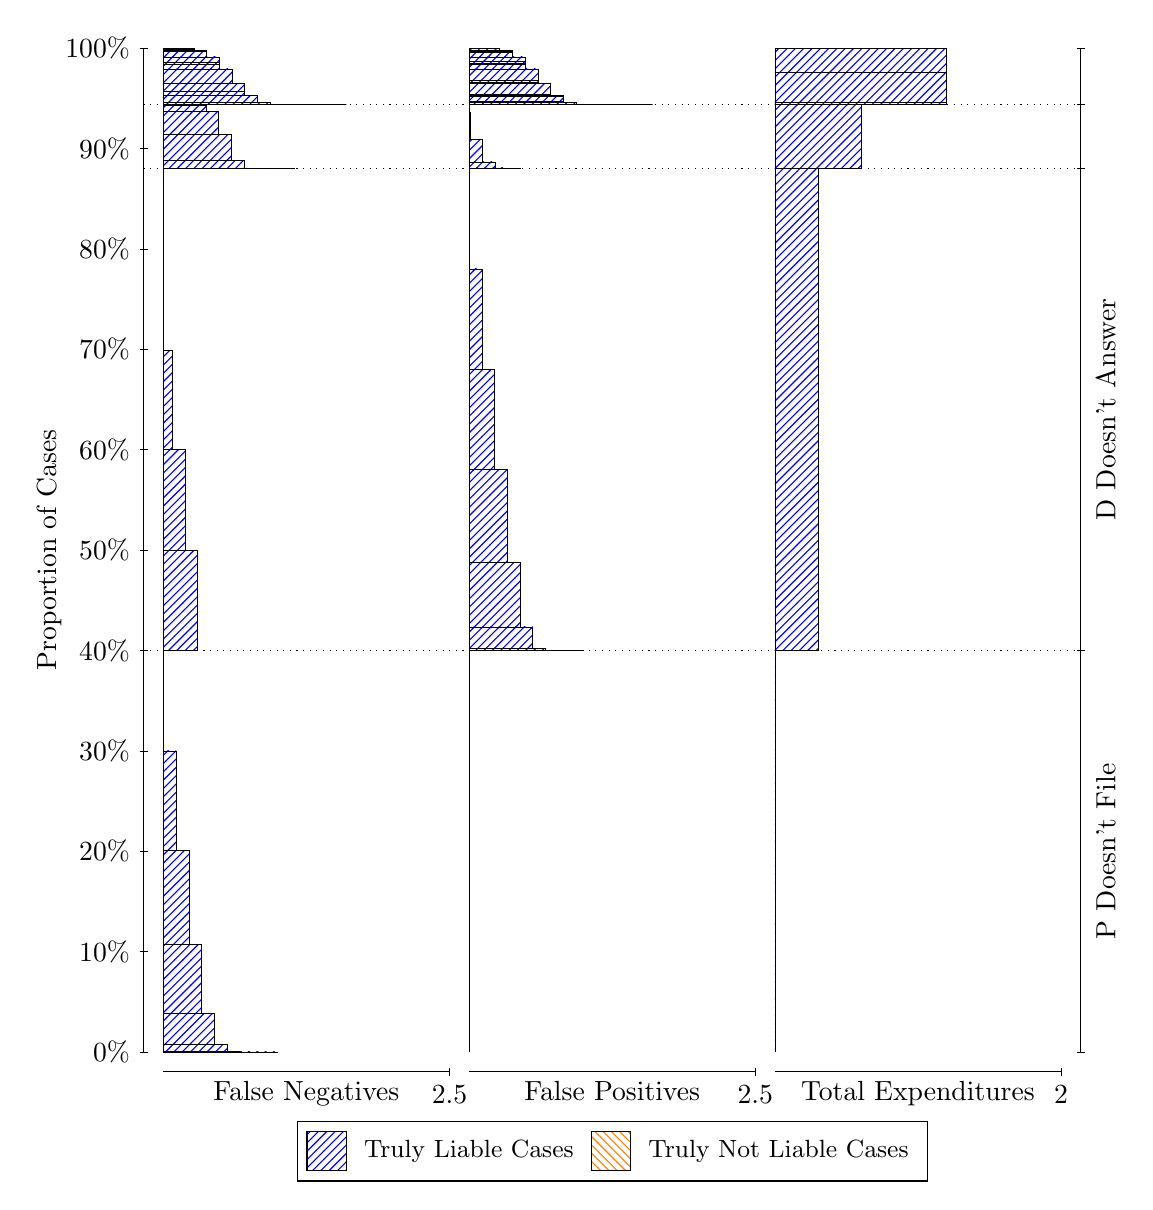
\begin{tikzpicture}
\draw[black, very thin] (1.5,1.75) -- (1.5,14.5);
\node[rotate=90, text=black, anchor=center] at (0.3, 8.125) {Proportion of Cases};
\draw[black, very thin] (1.45,1.75) -- (1.55,1.75);
\node[text=black, anchor=east] at (1.45, 1.75) {0\%};
\draw[black, very thin] (1.45,3.025) -- (1.55,3.025);
\node[text=black, anchor=east] at (1.45, 3.025) {10\%};
\draw[black, very thin] (1.45,4.3) -- (1.55,4.3);
\node[text=black, anchor=east] at (1.45, 4.3) {20\%};
\draw[black, very thin] (1.45,5.575) -- (1.55,5.575);
\node[text=black, anchor=east] at (1.45, 5.575) {30\%};
\draw[black, very thin] (1.45,6.85) -- (1.55,6.85);
\node[text=black, anchor=east] at (1.45, 6.85) {40\%};
\draw[black, very thin] (1.45,8.125) -- (1.55,8.125);
\node[text=black, anchor=east] at (1.45, 8.125) {50\%};
\draw[black, very thin] (1.45,9.4) -- (1.55,9.4);
\node[text=black, anchor=east] at (1.45, 9.4) {60\%};
\draw[black, very thin] (1.45,10.675) -- (1.55,10.675);
\node[text=black, anchor=east] at (1.45, 10.675) {70\%};
\draw[black, very thin] (1.45,11.95) -- (1.55,11.95);
\node[text=black, anchor=east] at (1.45, 11.95) {80\%};
\draw[black, very thin] (1.45,13.225) -- (1.55,13.225);
\node[text=black, anchor=east] at (1.45, 13.225) {90\%};
\draw[black, very thin] (1.45,14.5) -- (1.55,14.5);
\node[text=black, anchor=east] at (1.45, 14.5) {100\%};

\draw[black, very thin] (13.4,1.75) -- (13.4,14.5);
\draw[black, very thin] (13.35,1.75) -- (13.45,1.75);
\node[anchor=west] at (13.35, 1.75) {};
\draw[black, very thin] (13.35,6.8487) -- (13.45,6.8487);
\node[anchor=west] at (13.35, 6.8487) {};
\draw[black, very thin] (13.35,12.969) -- (13.45,12.969);
\node[anchor=west] at (13.35, 12.969) {};
\draw[black, very thin] (13.35,13.781) -- (13.45,13.781);
\node[anchor=west] at (13.35, 13.781) {};
\draw[black, very thin] (13.35,14.5) -- (13.45,14.5);
\node[anchor=west] at (13.35, 14.5) {};

\draw[black, very thin, pattern color=blue, pattern=north east lines] (1.75,1.75) rectangle (3.2033,1.75);
\draw[black, very thin, pattern color=blue, pattern=north east lines] (1.75,1.75) rectangle (3.0419,1.75);
\draw[black, very thin, pattern color=blue, pattern=north east lines] (1.75,1.75) rectangle (2.8804,1.7503);
\draw[black, very thin, pattern color=blue, pattern=north east lines] (1.75,1.7503) rectangle (2.7189,1.7582);
\draw[black, very thin, pattern color=blue, pattern=north east lines] (1.75,1.7582) rectangle (2.5574,1.8434);
\draw[black, very thin, pattern color=blue, pattern=north east lines] (1.75,1.8434) rectangle (2.3959,2.2368);
\draw[black, very thin, pattern color=blue, pattern=north east lines] (1.75,2.2368) rectangle (2.2344,3.1184);
\draw[black, very thin, pattern color=blue, pattern=north east lines] (1.75,3.1184) rectangle (2.073,4.3076);
\draw[black, very thin, pattern color=blue, pattern=north east lines] (1.75,4.3076) rectangle (1.9115,5.5742);
\draw[black, very thin, pattern color=orange, pattern=north west lines] (1.75,5.5742) rectangle (1.75,5.5742);
\draw[black, very thin, pattern color=blue, pattern=north east lines] (1.75,5.5742) rectangle (1.75,6.8487);
\draw[black, very thin, pattern color=blue, pattern=north east lines] (1.75,6.8487) rectangle (2.186,8.1237);
\draw[black, very thin, pattern color=blue, pattern=north east lines] (1.75,8.1237) rectangle (2.0245,9.3984);
\draw[black, very thin, pattern color=blue, pattern=north east lines] (1.75,9.3984) rectangle (1.863,10.665);
\draw[black, very thin, pattern color=orange, pattern=north west lines] (1.75,10.665) rectangle (1.75,10.665);
\draw[black, very thin, pattern color=blue, pattern=north east lines] (1.75,10.665) rectangle (1.75,12.969);
\draw[black, very thin, pattern color=blue, pattern=north east lines] (1.75,12.969) rectangle (3.4213,12.969);
\draw[black, very thin, pattern color=blue, pattern=north east lines] (1.75,12.969) rectangle (3.2599,12.969);
\draw[black, very thin, pattern color=blue, pattern=north east lines] (1.75,12.969) rectangle (3.0984,12.969);
\draw[black, very thin, pattern color=blue, pattern=north east lines] (1.75,12.969) rectangle (2.9369,12.974);
\draw[black, very thin, pattern color=blue, pattern=north east lines] (1.75,12.974) rectangle (2.7754,13.069);
\draw[black, very thin, pattern color=blue, pattern=north east lines] (1.75,13.069) rectangle (2.6139,13.407);
\draw[black, very thin, pattern color=blue, pattern=north east lines] (1.75,13.407) rectangle (2.4524,13.695);
\draw[black, very thin, pattern color=blue, pattern=north east lines] (1.75,13.695) rectangle (2.291,13.772);
\draw[black, very thin, pattern color=blue, pattern=north east lines] (1.75,13.772) rectangle (2.1295,13.78);
\draw[black, very thin, pattern color=blue, pattern=north east lines] (1.75,13.78) rectangle (1.968,13.781);
\draw[black, very thin, pattern color=orange, pattern=north west lines] (1.75,13.781) rectangle (1.75,13.781);
\draw[black, very thin, pattern color=blue, pattern=north east lines] (1.75,13.781) rectangle (4.0753,13.781);
\draw[black, very thin, pattern color=blue, pattern=north east lines] (1.75,13.781) rectangle (3.9139,13.781);
\draw[black, very thin, pattern color=blue, pattern=north east lines] (1.75,13.781) rectangle (3.7524,13.781);
\draw[black, very thin, pattern color=blue, pattern=north east lines] (1.75,13.781) rectangle (3.5909,13.781);
\draw[black, very thin, pattern color=blue, pattern=north east lines] (1.75,13.781) rectangle (3.4294,13.781);
\draw[black, very thin, pattern color=blue, pattern=north east lines] (1.75,13.781) rectangle (3.2679,13.783);
\draw[black, very thin, pattern color=blue, pattern=north east lines] (1.75,13.783) rectangle (3.2679,13.786);
\draw[black, very thin, pattern color=blue, pattern=north east lines] (1.75,13.786) rectangle (3.1064,13.813);
\draw[black, very thin, pattern color=blue, pattern=north east lines] (1.75,13.813) rectangle (3.1064,13.813);
\draw[black, very thin, pattern color=blue, pattern=north east lines] (1.75,13.813) rectangle (2.945,13.894);
\draw[black, very thin, pattern color=blue, pattern=north east lines] (1.75,13.894) rectangle (2.7835,13.953);
\draw[black, very thin, pattern color=blue, pattern=north east lines] (1.75,13.953) rectangle (2.7835,14.046);
\draw[black, very thin, pattern color=blue, pattern=north east lines] (1.75,14.046) rectangle (2.622,14.235);
\draw[black, very thin, pattern color=blue, pattern=north east lines] (1.75,14.235) rectangle (2.4605,14.294);
\draw[black, very thin, pattern color=blue, pattern=north east lines] (1.75,14.294) rectangle (2.4605,14.313);
\draw[black, very thin, pattern color=blue, pattern=north east lines] (1.75,14.313) rectangle (2.4605,14.387);
\draw[black, very thin, pattern color=blue, pattern=north east lines] (1.75,14.387) rectangle (2.299,14.458);
\draw[black, very thin, pattern color=blue, pattern=north east lines] (1.75,14.458) rectangle (2.299,14.467);
\draw[black, very thin, pattern color=blue, pattern=north east lines] (1.75,14.467) rectangle (2.1376,14.477);
\draw[black, very thin, pattern color=blue, pattern=north east lines] (1.75,14.477) rectangle (2.1376,14.48);
\draw[black, very thin, pattern color=blue, pattern=north east lines] (1.75,14.48) rectangle (2.1376,14.494);
\draw[black, very thin, pattern color=blue, pattern=north east lines] (1.75,14.494) rectangle (1.9761,14.499);
\draw[black, very thin, pattern color=blue, pattern=north east lines] (1.75,14.499) rectangle (1.9761,14.5);
\draw[black, very thin, pattern color=blue, pattern=north east lines] (1.75,14.5) rectangle (1.8146,14.5);
\draw[black, very thin, pattern color=blue, pattern=north east lines] (1.75,14.5) rectangle (1.8146,14.5);
\draw[black, very thin, pattern color=orange, pattern=north west lines] (1.75,14.5) rectangle (1.75,14.5);
\draw[black, very thin, pattern color=blue, pattern=north east lines] (1.75,14.5) rectangle (1.75,14.5);
\draw[black, very thin, pattern color=orange, pattern=north west lines] (5.6333,1.75) rectangle (5.6333,1.75);
\draw[black, very thin, pattern color=blue, pattern=north east lines] (5.6333,1.75) rectangle (5.6333,6.8487);
\draw[black, very thin, pattern color=orange, pattern=north west lines] (5.6333,6.8487) rectangle (7.0867,6.8487);
\draw[black, very thin, pattern color=blue, pattern=north east lines] (5.6333,6.8487) rectangle (7.0867,6.8487);
\draw[black, very thin, pattern color=blue, pattern=north east lines] (5.6333,6.8487) rectangle (6.9252,6.8487);
\draw[black, very thin, pattern color=blue, pattern=north east lines] (5.6333,6.8487) rectangle (6.7637,6.8493);
\draw[black, very thin, pattern color=blue, pattern=north east lines] (5.6333,6.8493) rectangle (6.6022,6.8756);
\draw[black, very thin, pattern color=blue, pattern=north east lines] (5.6333,6.8756) rectangle (6.4407,7.1476);
\draw[black, very thin, pattern color=blue, pattern=north east lines] (5.6333,7.1476) rectangle (6.2793,7.9703);
\draw[black, very thin, pattern color=blue, pattern=north east lines] (5.6333,7.9703) rectangle (6.1178,9.1527);
\draw[black, very thin, pattern color=blue, pattern=north east lines] (5.6333,9.1527) rectangle (5.9563,10.419);
\draw[black, very thin, pattern color=blue, pattern=north east lines] (5.6333,10.419) rectangle (5.7948,11.694);
\draw[black, very thin, pattern color=blue, pattern=north east lines] (5.6333,11.694) rectangle (5.6333,12.969);
\draw[black, very thin, pattern color=orange, pattern=north west lines] (5.6333,12.969) rectangle (6.2873,12.969);
\draw[black, very thin, pattern color=blue, pattern=north east lines] (5.6333,12.969) rectangle (6.2873,12.97);
\draw[black, very thin, pattern color=blue, pattern=north east lines] (5.6333,12.97) rectangle (6.1259,12.978);
\draw[black, very thin, pattern color=blue, pattern=north east lines] (5.6333,12.978) rectangle (5.9644,13.055);
\draw[black, very thin, pattern color=blue, pattern=north east lines] (5.6333,13.055) rectangle (5.8029,13.343);
\draw[black, very thin, pattern color=blue, pattern=north east lines] (5.6333,13.343) rectangle (5.6414,13.68);
\draw[black, very thin, pattern color=blue, pattern=north east lines] (5.6333,13.68) rectangle (5.6333,13.781);
\draw[black, very thin, pattern color=orange, pattern=north west lines] (5.6333,13.781) rectangle (7.9587,13.781);
\draw[black, very thin, pattern color=blue, pattern=north east lines] (5.6333,13.781) rectangle (7.9587,13.781);
\draw[black, very thin, pattern color=orange, pattern=north west lines] (5.6333,13.781) rectangle (7.7972,13.781);
\draw[black, very thin, pattern color=blue, pattern=north east lines] (5.6333,13.781) rectangle (7.7972,13.781);
\draw[black, very thin, pattern color=orange, pattern=north west lines] (5.6333,13.781) rectangle (7.6357,13.781);
\draw[black, very thin, pattern color=blue, pattern=north east lines] (5.6333,13.781) rectangle (7.6357,13.781);
\draw[black, very thin, pattern color=blue, pattern=north east lines] (5.6333,13.781) rectangle (7.4742,13.781);
\draw[black, very thin, pattern color=orange, pattern=north west lines] (5.6333,13.781) rectangle (7.4742,13.781);
\draw[black, very thin, pattern color=blue, pattern=north east lines] (5.6333,13.781) rectangle (7.4742,13.781);
\draw[black, very thin, pattern color=blue, pattern=north east lines] (5.6333,13.781) rectangle (7.3127,13.781);
\draw[black, very thin, pattern color=orange, pattern=north west lines] (5.6333,13.781) rectangle (7.3127,13.781);
\draw[black, very thin, pattern color=blue, pattern=north east lines] (5.6333,13.781) rectangle (7.3127,13.781);
\draw[black, very thin, pattern color=blue, pattern=north east lines] (5.6333,13.781) rectangle (7.1513,13.786);
\draw[black, very thin, pattern color=orange, pattern=north west lines] (5.6333,13.786) rectangle (7.1513,13.786);
\draw[black, very thin, pattern color=blue, pattern=north east lines] (5.6333,13.786) rectangle (7.1513,13.786);
\draw[black, very thin, pattern color=blue, pattern=north east lines] (5.6333,13.786) rectangle (6.9898,13.789);
\draw[black, very thin, pattern color=orange, pattern=north west lines] (5.6333,13.789) rectangle (6.9898,13.789);
\draw[black, very thin, pattern color=blue, pattern=north east lines] (5.6333,13.789) rectangle (6.9898,13.813);
\draw[black, very thin, pattern color=blue, pattern=north east lines] (5.6333,13.813) rectangle (6.9898,13.813);
\draw[black, very thin, pattern color=blue, pattern=north east lines] (5.6333,13.813) rectangle (6.9898,13.813);
\draw[black, very thin, pattern color=blue, pattern=north east lines] (5.6333,13.813) rectangle (6.8283,13.823);
\draw[black, very thin, pattern color=orange, pattern=north west lines] (5.6333,13.823) rectangle (6.8283,13.823);
\draw[black, very thin, pattern color=blue, pattern=north east lines] (5.6333,13.823) rectangle (6.8283,13.893);
\draw[black, very thin, pattern color=blue, pattern=north east lines] (5.6333,13.893) rectangle (6.8283,13.894);
\draw[black, very thin, pattern color=blue, pattern=north east lines] (5.6333,13.894) rectangle (6.6668,13.894);
\draw[black, very thin, pattern color=blue, pattern=north east lines] (5.6333,13.894) rectangle (6.6668,13.914);
\draw[black, very thin, pattern color=orange, pattern=north west lines] (5.6333,13.914) rectangle (6.6668,13.914);
\draw[black, very thin, pattern color=blue, pattern=north east lines] (5.6333,13.914) rectangle (6.6668,14.046);
\draw[black, very thin, pattern color=blue, pattern=north east lines] (5.6333,14.046) rectangle (6.5053,14.067);
\draw[black, very thin, pattern color=orange, pattern=north west lines] (5.6333,14.067) rectangle (6.5053,14.067);
\draw[black, very thin, pattern color=blue, pattern=north east lines] (5.6333,14.067) rectangle (6.5053,14.092);
\draw[black, very thin, pattern color=blue, pattern=north east lines] (5.6333,14.092) rectangle (6.5053,14.235);
\draw[black, very thin, pattern color=blue, pattern=north east lines] (5.6333,14.235) rectangle (6.3439,14.292);
\draw[black, very thin, pattern color=blue, pattern=north east lines] (5.6333,14.292) rectangle (6.3439,14.309);
\draw[black, very thin, pattern color=blue, pattern=north east lines] (5.6333,14.309) rectangle (6.3439,14.33);
\draw[black, very thin, pattern color=blue, pattern=north east lines] (5.6333,14.33) rectangle (6.3439,14.387);
\draw[black, very thin, pattern color=blue, pattern=north east lines] (5.6333,14.387) rectangle (6.1824,14.448);
\draw[black, very thin, pattern color=blue, pattern=north east lines] (5.6333,14.448) rectangle (6.1824,14.457);
\draw[black, very thin, pattern color=blue, pattern=north east lines] (5.6333,14.457) rectangle (6.1824,14.467);
\draw[black, very thin, pattern color=blue, pattern=north east lines] (5.6333,14.467) rectangle (6.0209,14.47);
\draw[black, very thin, pattern color=blue, pattern=north east lines] (5.6333,14.47) rectangle (6.0209,14.473);
\draw[black, very thin, pattern color=blue, pattern=north east lines] (5.6333,14.473) rectangle (6.0209,14.494);
\draw[black, very thin, pattern color=blue, pattern=north east lines] (5.6333,14.494) rectangle (6.0209,14.494);
\draw[black, very thin, pattern color=blue, pattern=north east lines] (5.6333,14.494) rectangle (5.8594,14.497);
\draw[black, very thin, pattern color=blue, pattern=north east lines] (5.6333,14.497) rectangle (5.8594,14.5);
\draw[black, very thin, pattern color=blue, pattern=north east lines] (5.6333,14.5) rectangle (5.6979,14.5);
\draw[black, very thin, pattern color=blue, pattern=north east lines] (5.6333,14.5) rectangle (5.6979,14.5);
\draw[black, very thin, pattern color=blue, pattern=north east lines] (5.6333,14.5) rectangle (5.6979,14.5);
\draw[black, very thin, pattern color=blue, pattern=north east lines] (5.6333,14.5) rectangle (5.6333,14.5);
\draw[black, very thin, pattern color=orange, pattern=north west lines] (9.5167,1.75) rectangle (9.5167,1.75);
\draw[black, very thin, pattern color=blue, pattern=north east lines] (9.5167,1.75) rectangle (9.5167,6.8487);
\draw[black, very thin, pattern color=orange, pattern=north west lines] (9.5167,6.8487) rectangle (10.062,6.8487);
\draw[black, very thin, pattern color=blue, pattern=north east lines] (9.5167,6.8487) rectangle (10.062,12.969);
\draw[black, very thin, pattern color=orange, pattern=north west lines] (9.5167,12.969) rectangle (10.607,12.969);
\draw[black, very thin, pattern color=blue, pattern=north east lines] (9.5167,12.969) rectangle (10.607,13.781);
\draw[black, very thin, pattern color=orange, pattern=north west lines] (9.5167,13.781) rectangle (11.697,13.781);
\draw[black, very thin, pattern color=blue, pattern=north east lines] (9.5167,13.781) rectangle (11.697,13.811);
\draw[black, very thin, pattern color=orange, pattern=north west lines] (9.5167,13.811) rectangle (11.697,13.811);
\draw[black, very thin, pattern color=blue, pattern=north east lines] (9.5167,13.811) rectangle (11.697,14.189);
\draw[black, very thin, pattern color=orange, pattern=north west lines] (9.5167,14.189) rectangle (11.697,14.189);
\draw[black, very thin, pattern color=blue, pattern=north east lines] (9.5167,14.189) rectangle (11.697,14.5);
\draw[black, dotted] (1.5,6.8487) -- (13.4,6.8487);
\draw[black, dotted] (1.5,12.969) -- (13.4,12.969);
\draw[black, dotted] (1.5,13.781) -- (13.4,13.781);
\draw[black, very thin] (1.75,1.5) -- (5.3833,1.5);
\node[text=black, anchor=north] at (3.5667, 1.5) {False Negatives};
\draw[black, very thin] (5.3833,1.45) -- (5.3833,1.55);
\node[text=black, anchor=north] at (5.3833, 1.45) {2.5};

\draw[black, very thin] (5.6333,1.5) -- (9.2667,1.5);
\node[text=black, anchor=north] at (7.45, 1.5) {False Positives};
\draw[black, very thin] (9.2667,1.45) -- (9.2667,1.55);
\node[text=black, anchor=north] at (9.2667, 1.45) {2.5};

\draw[black, very thin] (9.5167,1.5) -- (13.15,1.5);
\node[text=black, anchor=north] at (11.333, 1.5) {Total Expenditures};
\draw[black, very thin] (13.15,1.45) -- (13.15,1.55);
\node[text=black, anchor=north] at (13.15, 1.45) {2};

\node[text=black, centered, rotate=90] at (13.72, 4.2994) {P Doesn't File};
\node[text=black, centered, rotate=90] at (13.72, 9.9089) {D Doesn't Answer};



\draw (7.449999999999999,1.5) node[draw=none] (baseCoordinate) {};
\begin{scope}[align=center]
        \matrix[scale=0.5, draw=black, below=0.5cm of baseCoordinate, nodes={draw}, column sep=0.1cm]{
            \node[rectangle, draw, minimum width=0.5cm, minimum height=0.5cm, pattern color=blue, pattern=north east lines] {}; &
            \node[draw=none, font=\small, text=black] (B) {Truly Liable Cases}; &
            \node[rectangle, draw, minimum width=0.5cm, minimum height=0.5cm, pattern color=orange, pattern=north west lines] {}; &
            \node[draw=none, font=\small, text=black] (B) {Truly Not Liable Cases}; \\
            };
\end{scope}

\end{tikzpicture}
\end{document}